\documentclass[11pt]{article}

\usepackage[margin=1in]{geometry}
\usepackage{amsmath,amssymb,mathtools}
\usepackage{graphicx}
\usepackage{booktabs}
\usepackage{hyperref}
\usepackage{enumitem}
\usepackage{xcolor}
\usepackage{microtype}

\hypersetup{
  colorlinks=true,
  linkcolor=blue!55!black,
  citecolor=blue!55!black,
  urlcolor=blue!55!black
}

\newcommand{\R}{\mathbb{R}}
\newcommand{\N}{\mathcal{N}}
\newcommand{\E}{\mathcal{E}}
\newcommand{\one}{\mathbf{1}}

\title{PHATE, Symmetric kNN, Mutual kNN, and Intersection kNN Graph Constructions}
\author{gflow development note}
\date{\today}

\begin{document}
\maketitle

\begin{abstract}
This note gives a self-contained description of several graph constructions on a finite data
set: the PHATE adaptive affinity graph, the symmetric or union k-nearest-neighbor graph, the
mutual k-nearest-neighbor graph, and the intersection k-nearest-neighbor graph.  The main
point is that the PHATE graph with additive symmetrization has an adaptive-radius edge condition
\[
  d_{ij} \le r_\tau \max(\sigma_i,\sigma_j),
\]
where \(r_\tau=(-\log \tau)^{1/a}\).  Without the factor \(r_\tau\), this is the standard
symmetric kNN, or union kNN, support.  In contrast, the mutual kNN graph has the smaller
radius condition
\[
  d_{ij}\le \min(\sigma_i,\sigma_j)
\]
when there are no nearest-neighbor ties.  The intersection kNN graph is not a radius graph:
it connects points whose closed k-neighborhoods have nonempty intersection.  Thus mutual kNN
is naturally contained in both the PHATE support under matching conventions and the closed
intersection kNN support, but PHATE and intersection kNN are not generally nested.  Figures
illustrate these distinctions on roots of unity, a larger uniform circle, and noisy circles
constructed with a sample Fermat distance.
\end{abstract}

\section{Setup and conventions}

Let
\[
  X=\{x_1,\ldots,x_n\}\subset \R^p
\]
be a finite data set, and let \(D=(d_{ij})\) be a symmetric nonnegative distance matrix on
\(X\), with \(d_{ii}=0\).  In Euclidean examples,
\[
  d_{ij}=\lVert x_i-x_j\rVert_2.
\]
In the noisy-circle examples below, \(D\) is instead a sample Fermat distance computed from
the observed points.

For a fixed integer \(k\in\{1,\ldots,n-1\}\), define \(N_k(i)\) to be the set of the \(k\)
nearest neighbors of \(x_i\), excluding \(x_i\) itself, and define the corresponding closed
k-neighborhood
\[
  \widehat{N}_k(i)=\{i\}\cup N_k(i).
\]
Unless otherwise noted, ties are resolved by vertex index.  This tie convention is only
needed for finite examples with exact symmetry; the formulae below are cleanest when there
are no ties.

Define the local k-neighbor radius
\[
  \sigma_i=d_{i,(k)},
\]
where \(d_{i,(k)}\) is the distance from \(x_i\) to its \(k\)-th non-self nearest neighbor.
Equivalently, in the no-tie case,
\[
  j\in N_k(i)
  \quad\Longleftrightarrow\quad
  d_{ij}\le \sigma_i.
\]

\section{Terminology}

The following names are used in this note.  We recommend using \textbf{sKNN} as the primary
abbreviation for the graph with edge rule \(d_{ij}\le \max(\sigma_i,\sigma_j)\), because
``symmetric kNN graph'' is the common name in graph-based learning and spectral clustering.
The abbreviation \textbf{uKNN} is also useful when the point is to emphasize that this graph
is the union, or OR-symmetrization, of directed kNN edges.

\begin{center}
\begin{tabular}{lll}
\toprule
Name & Abbreviation & Edge rule, no ties \\
\midrule
Directed kNN & dKNN & \(j\in N_k(i)\) as a directed edge \(i\to j\) \\
Symmetric kNN / union kNN & sKNN / uKNN & \(d_{ij}\le \max(\sigma_i,\sigma_j)\) \\
Mutual kNN & mKNN & \(d_{ij}\le \min(\sigma_i,\sigma_j)\) \\
Intersection kNN & ikNN & \(\widehat{N}_k(i)\cap\widehat{N}_k(j)\ne\varnothing\) \\
PHATE support & PHATE & \(d_{ij}\le r_\tau\max(\sigma_i,\sigma_j)\) \\
\bottomrule
\end{tabular}
\end{center}

\section{Directed and symmetric kNN graphs}

The raw kNN graph is naturally a directed graph:
\[
  i\to j
  \quad\Longleftrightarrow\quad
  j\in N_k(i).
\]
It is called ``raw'' here only to distinguish the directed neighbor-search result from later
undirected graph constructions.  The directed graph need not be symmetric: \(j\) can be one
of the \(k\) nearest neighbors of \(i\) without \(i\) being one of the \(k\) nearest neighbors
of \(j\).

The symmetric kNN graph, also called the union kNN graph, makes the directed kNN relation
undirected by the OR rule:
\[
  \{i,j\}\in E_{\mathrm{sKNN}}
  \quad\Longleftrightarrow\quad
  j\in N_k(i)\quad\text{or}\quad i\in N_k(j).
\]
Equivalently, in the no-tie case,
\[
  \{i,j\}\in E_{\mathrm{sKNN}}
  \quad\Longleftrightarrow\quad
  d_{ij}\le \max(\sigma_i,\sigma_j).
\]
This graph is widely used in graph-based learning.  The contrast between symmetric kNN and
mutual kNN is standard in spectral clustering and related graph-construction work: sKNN is
usually better connected, while mKNN is more conservative and can suppress edges across
sampling-density changes.

\section{Mutual kNN graph}

The mutual k-nearest-neighbor graph, denoted \(G_{\mathrm{mKNN}}=(V,E_{\mathrm{mKNN}})\),
has vertex set \(V=\{1,\ldots,n\}\).  An undirected edge \(\{i,j\}\), \(i\ne j\), is present
if and only if
\[
  j\in \widehat{N}_k(i)
  \quad\text{and}\quad
  i\in \widehat{N}_k(j).
\]
This matches gflow's native mKNN implementation: the backend kNN search includes the query
point itself, so the R wrapper asks for \(k+1\) backend neighbors in order to represent
\(\widehat{N}_k(i)\).  Since \(i\ne j\), the closed-neighborhood condition is equivalent to
the more familiar open-neighborhood reciprocal rule
\[
  j\in N_k(i)
  \quad\text{and}\quad
  i\in N_k(j).
\]
When there are no ties, this is equivalent to
\[
  d_{ij}\le \sigma_i
  \quad\text{and}\quad
  d_{ij}\le \sigma_j,
\]
or
\[
  d_{ij}\le \min(\sigma_i,\sigma_j).
\]
Thus mKNN is a conservative reciprocal-neighborhood graph.  It keeps edges only when both
endpoints regard each other as locally close.

\section{Intersection kNN graph}

The intersection k-nearest-neighbor graph, denoted \(G_{\mathrm{ikNN}}=(V,E_{\mathrm{ikNN}})\),
also uses the closed k-neighborhoods \(\widehat{N}_k(i)\).  This matches gflow's native ikNN
implementation for the same backend reason as mKNN.  Here, however, closing the neighborhood
does change the edge predicate.  The graph has an edge \(\{i,j\}\) if the two closed
k-neighborhoods share at least one point:
\[
  \{i,j\}\in E_{\mathrm{ikNN}}
  \quad\Longleftrightarrow\quad
  \widehat{N}_k(i)\cap \widehat{N}_k(j)\ne \varnothing.
\]
This is not a direct radius condition on \(d_{ij}\).  Two points can be connected because
they both regard a third point as nearby, even if \(i\) and \(j\) are not mutually close.
The closed-neighborhood convention also means that every mKNN edge is an ikNN edge: if
\(j\in N_k(i)\) and \(i\in N_k(j)\), then both \(i\) and \(j\) lie in
\(\widehat{N}_k(i)\cap\widehat{N}_k(j)\).  Consequently, \(G_{\mathrm{ikNN}}\) can be much
denser than mKNN or PHATE, but it need not contain PHATE in every finite configuration.

In gflow's native ikNN implementation, the graph also carries an edge weight.  For an ikNN
edge \(\{i,j\}\), the stored native length is an intersection-mediated detour length of the
form
\[
  \ell_{ij}^{\mathrm{ikNN}}
  =
  \min_{c\in \widehat{N}_k(i)\cap\widehat{N}_k(j)}
  \{d_{ic}+d_{jc}\}.
\]
This is a length, not a similarity.  If the intersection contains one of the endpoints,
then this minimum can equal the direct chord length \(d_{ij}\); otherwise it is an
intersection-mediated detour length.

\section{PHATE adaptive affinity graph}

PHATE constructs a directed adaptive affinity before symmetrization.  For each point \(i\),
let
\[
  \sigma_i=b\,d_{i,(k)}
\]
where \(b>0\) is a bandwidth scale.  In the examples below \(b=1\).  For decay parameter
\(a>0\), define
\[
  A_{ij}
  =
  \exp\left[-\left(\frac{d_{ij}}{\sigma_i}\right)^a\right],
  \qquad
  A_{ii}=1.
\]
PHATE then thresholds small directed affinities:
\[
  A_{ij}=0
  \quad\text{if}\quad
  A_{ij}<\tau,
\]
where \(\tau=10^{-4}\) is the default threshold used in these examples.

The directed threshold condition is
\[
  \exp\left[-\left(\frac{d_{ij}}{\sigma_i}\right)^a\right]\ge \tau.
\]
Taking logarithms gives
\[
  d_{ij}\le r_\tau \sigma_i,
  \qquad
  r_\tau=(-\log\tau)^{1/a}.
\]
For \(a=40\) and \(\tau=10^{-4}\),
\[
  r_\tau=(-\log 10^{-4})^{1/40}\approx 1.057.
\]
So in one directed row, PHATE keeps nearly the same radius as the k-nearest-neighbor
radius when \(a=40\).  Smaller \(a\) produces a larger effective threshold radius.

PHATE then symmetrizes the directed kernel.  With additive symmetrization,
\[
  K_{ij}=\frac{A_{ij}+A_{ji}}{2}.
\]
The undirected PHATE support is
\[
  E_{\mathrm{PHATE}}
  =
  \{\{i,j\}: i<j,\ K_{ij}>0\}.
\]
Because \(K_{ij}>0\) if and only if at least one directed affinity survives thresholding,
\[
  \{i,j\}\in E_{\mathrm{PHATE}}
  \quad\Longleftrightarrow\quad
  d_{ij}\le r_\tau\sigma_i
  \quad\text{or}\quad
  d_{ij}\le r_\tau\sigma_j.
\]
Equivalently,
\[
  \{i,j\}\in E_{\mathrm{PHATE}}
  \quad\Longleftrightarrow\quad
  d_{ij}\le r_\tau\max(\sigma_i,\sigma_j).
\]
Thus the PHATE support is an adaptive-affinity, threshold-inflated version of the symmetric
kNN support.  When \(a=40\), \(\tau=10^{-4}\), and \(b=1\), the inflation factor is only
about \(1.057\); with smaller decay values it becomes visibly larger.
If both directed affinities survive, \(K_{ij}\) is their average.  If only one direction
survives, \(K_{ij}\) is half of the surviving directed affinity.

Finally, PHATE row-normalizes \(K\) to obtain a Markov diffusion operator
\[
  P_{ij}=\frac{K_{ij}}{\sum_{\ell=1}^n K_{i\ell}}.
\]
The graph support discussed in this note is the nonzero off-diagonal support of \(K\), not
the row-normalized matrix \(P\).

\section{Relations among the graph supports}

Assume that the constructions use the same distance matrix \(D\), the same \(k\),
bandwidth scale \(b=1\), additive PHATE symmetrization, and no nearest-neighbor ties.
Then
\[
  \{i,j\}\in E_{\mathrm{mKNN}}
  \quad\Longleftrightarrow\quad
  d_{ij}\le \min(\sigma_i,\sigma_j).
\]
Since
\[
  \min(\sigma_i,\sigma_j)
  \le
  r_\tau \max(\sigma_i,\sigma_j)
\]
for \(r_\tau\ge 1\), we have
\[
  E_{\mathrm{mKNN}}\subseteq E_{\mathrm{PHATE}}.
\]
This inclusion is the precise sense in which PHATE is less restrictive than mKNN.
More specifically,
\[
  E_{\mathrm{mKNN}}\subseteq E_{\mathrm{sKNN}},
\]
because the AND rule implies the OR rule.  With \(r_\tau\ge 1\), the symmetric kNN graph is
contained in the PHATE support:
\[
  E_{\mathrm{sKNN}}\subseteq E_{\mathrm{PHATE}}.
\]
For PHATE defaults this containment is often close to equality, but the extra factor
\(r_\tau\) can add edges just beyond the local kNN radius.

However, \(E_{\mathrm{ikNN}}\) is not governed by a direct radius threshold.  It is governed
by the set condition
\[
  \widehat{N}_k(i)\cap \widehat{N}_k(j)\ne\varnothing.
\]
Therefore one should not write a general nesting relation such as
\[
  E_{\mathrm{PHATE}}\subseteq E_{\mathrm{ikNN}}
  \quad\text{or}\quad
  E_{\mathrm{ikNN}}\subseteq E_{\mathrm{PHATE}}.
\]
In many sampled manifolds, ikNN has more edges than PHATE because many point pairs share
neighbors.  But this is an empirical edge-count tendency, not a theorem of set inclusion.

\section{Notes on usage in applications}

In many applied workflows, especially single-cell analysis, the first computational object is
a kNN search result: for each observation \(i\), store the directed list \(N_k(i)\).  This is
the raw directed kNN graph \(i\to j\).  It is not yet one unique undirected graph.  Different
methods then turn the directed lists into graph objects in different ways.

One common choice is a symmetric or union kNN support, where an undirected edge is present if
either endpoint appears in the other's directed neighbor list.  This is the sKNN/uKNN graph
defined above.  UMAP-style neighbor graphs are closely related: they build directed local
fuzzy membership strengths and combine the two directed memberships through a fuzzy union.
If one ignores the exact fuzzy weights and only asks whether an edge can be present, this is
an OR-style symmetrization of local neighbor relations.

Single-cell tools also often construct a shared nearest-neighbor graph, usually abbreviated
SNN.  The SNN graph should not be confused with sKNN.  SNN weights are based on neighborhood
overlap, for example a Jaccard-type score such as
\[
  w^{\mathrm{SNN}}_{ij}
  =
  \frac{\lvert N_k(i)\cap N_k(j)\rvert}
       {\lvert N_k(i)\cup N_k(j)\rvert},
\]
possibly using closed neighborhoods or implementation-specific variants.  Seurat's
\texttt{FindNeighbors()} workflow, for example, constructs a kNN graph and can then compute
an SNN graph by comparing the neighbor lists.  This SNN weighting step is conceptually closer
to shared-neighborhood ideas than to the max-\(\sigma\) radius rule.  The max-\(\sigma\) graph
is the binary symmetric/union kNN support; SNN is an overlap-weighted graph derived from
neighbor-list intersections.

\section{kNN plus MST connectivity augmentation}

A recurring practical problem is that a neighborhood graph can be disconnected.  This is not
necessarily an error: disconnected components can be meaningful evidence that the data contain
separate geometric pieces.  However, some downstream procedures, including graph geodesic
distances, spectral embeddings, diffusion processes, and Isomap-style projection methods, may
require a connected graph.  A standard way to enforce connectedness while changing the local
graph as little as possible is a kNN plus MST construction.

Let \(G=(V,E)\) be an initial undirected neighborhood graph, such as sKNN, with connected
components
\[
  C_1,\ldots,C_m.
\]
If \(m=1\), no augmentation is needed.  If \(m>1\), form the complete component graph
\[
  G_C=(\{1,\ldots,m\},E_C),
\]
where the edge between components \(C_a\) and \(C_b\) is weighted by the shortest data-space
edge that could connect them:
\[
  w_{ab}
  =
  \min_{i\in C_a,\ j\in C_b} d_{ij}.
\]
Choose one attaining pair
\[
  (i^\ast_{ab},j^\ast_{ab})
  \in
  \arg\min_{i\in C_a,\ j\in C_b} d_{ij}.
\]
Then compute a minimum spanning tree \(T_C\) of the component graph \(G_C\) and add to \(G\)
the corresponding data-space bridge edges
\[
  \{i^\ast_{ab},j^\ast_{ab}\},
  \qquad
  (a,b)\in T_C.
\]
This adds exactly \(m-1\) edges, which is the smallest possible number of edges that can
connect \(m\) components.  For example, if the initial graph has three connected components,
the component-MST augmentation adds two bridge edges, not all three pairwise component
bridges.  The selected bridges minimize total added bridge length among all ways to connect
the component graph by a tree.

This construction is closely related to what is often called a kNN-MST graph: take a kNN-type
neighborhood graph and augment it with MST edges to avoid disconnected supports.  A slightly
different but also common variant computes a global MST on all data points and unions that
MST with the kNN graph.  The global-MST union also guarantees connectedness, but it can add
within-component MST edges that are not needed merely to connect the components.  For this
reason, the component-MST augmentation is the more minimal choice when the goal is only to
make an already constructed graph connected.

This report's corresponding gflow implementation is \texttt{create.sknn.graph()}.  It builds
the sKNN/uKNN support in C++ and optionally augments disconnected graphs with MST bridges:
\[
\begin{array}{ll}
\texttt{connect.components = FALSE} & \text{return the unaugmented sKNN graph,}\\
\texttt{connect.method = "component.mst"} & \text{add the component-MST bridge edges,}\\
\texttt{connect.method = "global.mst"} & \text{union the graph with the full Euclidean MST.}
\end{array}
\]
The default is not to force connectedness, because disconnectedness can itself be a useful
diagnostic.  When connectedness is required for downstream geodesic or spectral methods,
\texttt{connect.method = "component.mst"} is the recommended first choice.

\section{Root-of-unity examples}

This section shows deterministic finite examples on the unit circle.  The points are
\[
  x_m=(\cos(2\pi m/n),\sin(2\pi m/n)),
  \qquad
  m=0,\ldots,n-1.
\]
For \(n=3,4,5\), we use \(k=2\), \(a=40\), and \(\tau=10^{-4}\).  For \(n=100\), we use
\(k=10\).  All graph constructions use Euclidean distances.  Each figure shows PHATE,
sKNN, mKNN, and ikNN supports in that order.

\subsection{Three roots of unity}

For \(n=3\) and \(k=2\), every point has the other two points as its two nearest neighbors.
Therefore
\[
  N_2(i)=\{1,2,3\}\setminus\{i\}.
\]
Every pair is mutually 2-nearest, so mKNN is the complete graph \(K_3\).  Since every
distance equals \(\sigma_i\), every pair also satisfies
\[
  d_{ij}\le r_\tau \sigma_i
\]
in both directions, so PHATE is also \(K_3\).  Finally, any two distinct vertices have
neighbor sets with nonempty intersection, so ikNN is \(K_3\) as well.

\begin{figure}[htbp]
  \centering
  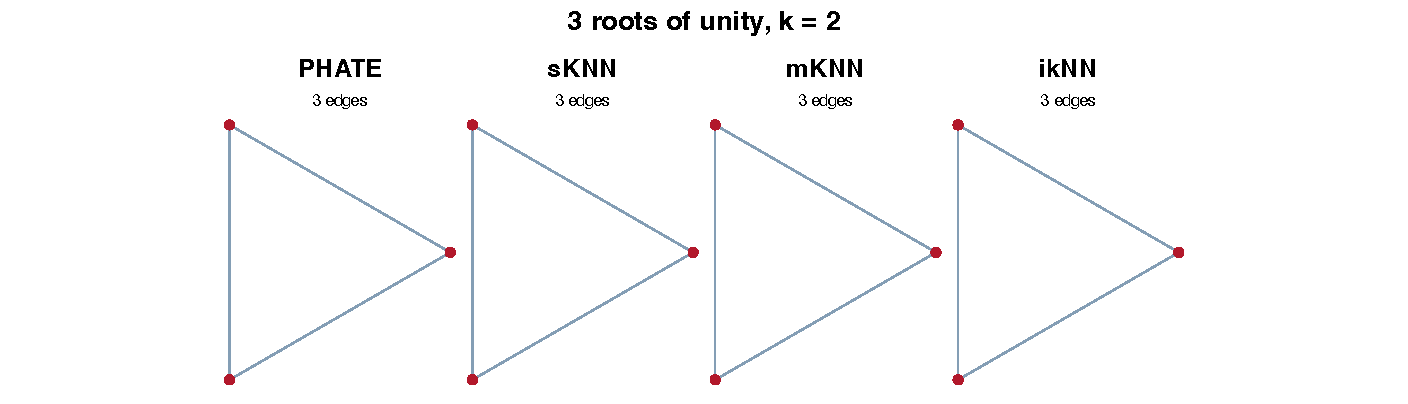
\includegraphics[width=\linewidth]{figures/roots_n3_k2.pdf}
  \caption{Three roots of unity with \(k=2\).  All four constructions produce the complete graph.}
\end{figure}

\subsection{Four and five roots of unity}

For \(n=4\) and \(k=2\), mKNN and PHATE both recover the cycle edges.  The closed-neighborhood
ikNN graph is complete: adjacent vertices share their endpoints through the closed
neighborhood convention, and opposite vertices share adjacent nearest neighbors.  This
example is useful because it shows how quickly ikNN can densify even when PHATE remains a
local adaptive-radius graph.

\begin{figure}[htbp]
  \centering
  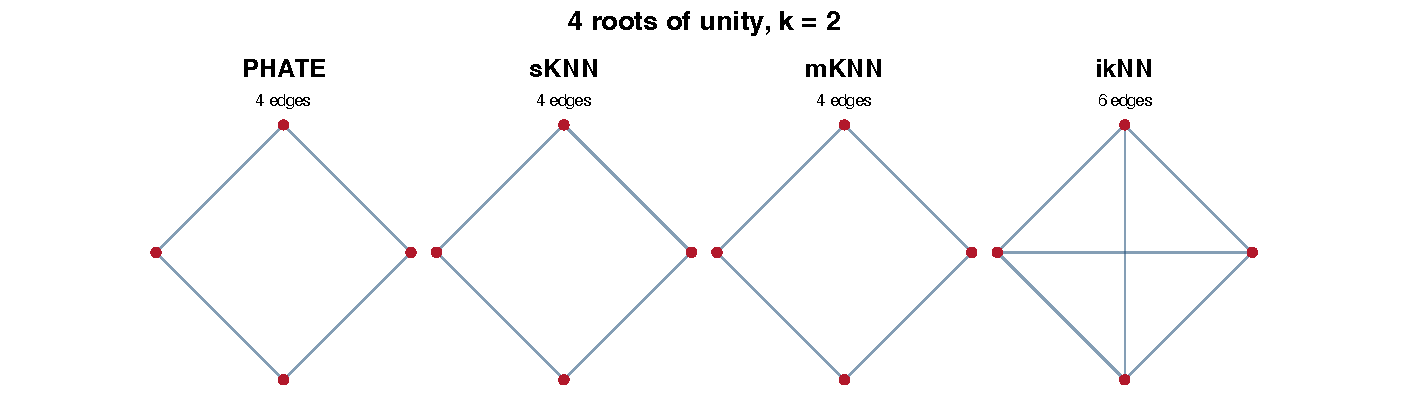
\includegraphics[width=\linewidth]{figures/roots_n4_k2.pdf}
  \caption{Four roots of unity with \(k=2\).  PHATE, sKNN, and mKNN produce the cycle, while closed-neighborhood ikNN produces the complete graph.}
\end{figure}

For \(n=5\) and \(k=2\), PHATE and mKNN again recover the adjacent cycle.  The closed-neighborhood
ikNN graph is again complete: cycle edges are present through endpoint sharing and the
remaining pairs share one intermediate nearest neighbor around the circle.

\begin{figure}[htbp]
  \centering
  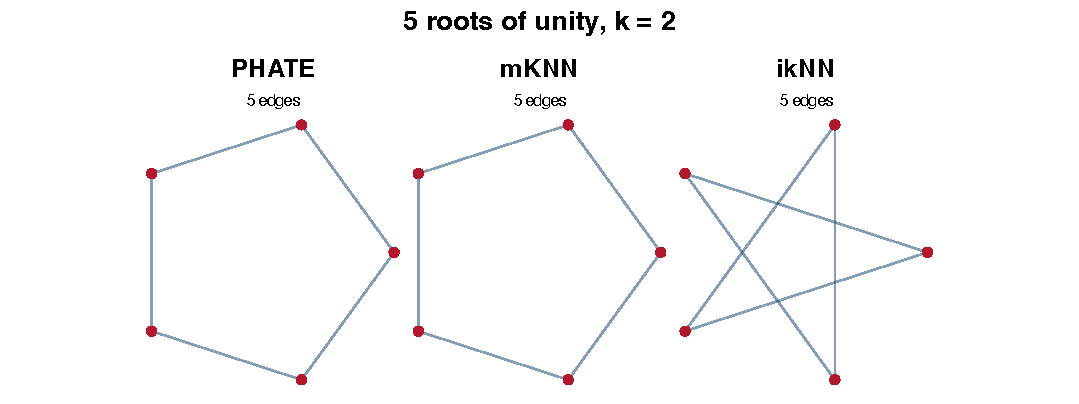
\includegraphics[width=\linewidth]{figures/roots_n5_k2.pdf}
  \caption{Five roots of unity with \(k=2\).  PHATE, sKNN, and mKNN keep adjacent circle edges; closed-neighborhood ikNN connects every pair.}
\end{figure}

\subsection{One hundred roots of unity}

For \(n=100\) and \(k=10\), PHATE remains close to the sKNN local circular band because
\(r_\tau\approx1.057\).  mKNN is the reciprocal-neighborhood graph.  ikNN is visibly denser
because many pairs share at least one of their ten nearest neighbors.

\begin{figure}[htbp]
  \centering
  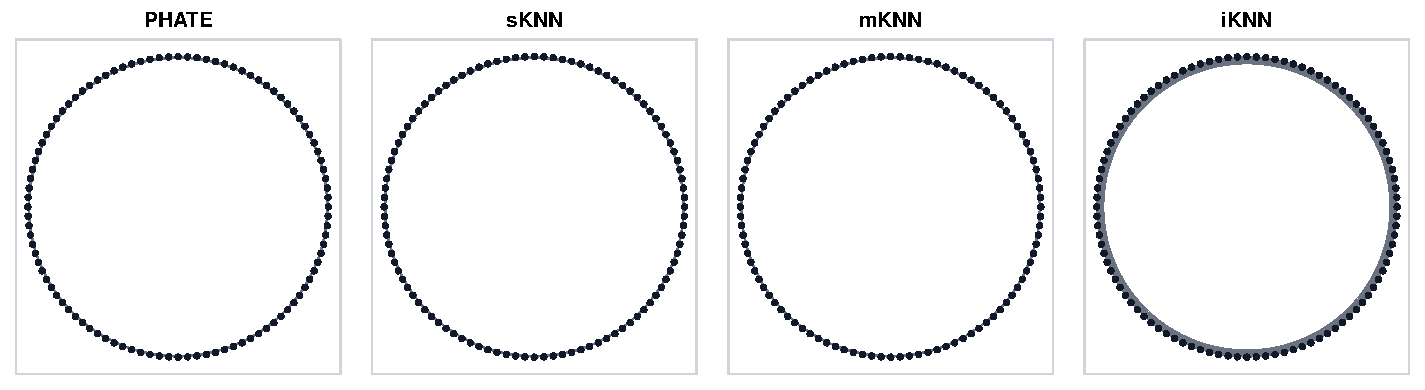
\includegraphics[width=\linewidth]{figures/roots_n100_k10.pdf}
  \caption{One hundred roots of unity with \(k=10\).  PHATE is close to sKNN, while ikNN is denser because it is based on shared neighborhoods rather than reciprocal or adaptive-radius proximity.}
\end{figure}

\section{Noisy circle with sample Fermat distance}

The term \emph{Fermat distance} is standard in the density-aware metric learning literature.
For a sample \(X\), a common discrete version is a shortest-path metric whose edge costs are
powers of Euclidean lengths.  In the examples here, we first build a base kNN graph on the
observed noisy circle and assign each base edge \(\{i,j\}\) the cost
\[
  c_{ij}=\lVert x_i-x_j\rVert_2^\alpha,
\]
with \(\alpha=2\).  The sample Fermat distance is then
\[
  d_F(i,j)=\min_{\gamma:i\leadsto j}\sum_{\{u,v\}\in\gamma} c_{uv}.
\]
This is a graph-based sample version of Fermat-type distances: when \(\alpha>1\), long
single jumps are penalized more heavily, and shortest paths tend to follow chains of nearby
sample points.  We then construct PHATE, sKNN, mKNN, and ikNN graphs using \(d_F\) as the
input distance matrix.  The figures are drawn in the original noisy Euclidean coordinates so
that the supports can be inspected visually.

Under each noisy-circle graph comparison we also show a PHATE-versus-sKNN diagnostic row.
The first diagnostic panel highlights
\[
  E_{\mathrm{PHATE}}\setminus E_{\mathrm{sKNN}},
\]
the edges added by the PHATE threshold inflation.  The second highlights
\[
  E_{\mathrm{sKNN}}\setminus E_{\mathrm{PHATE}},
\]
which should usually be empty under matching no-tie assumptions and \(r_\tau\ge1\), but is
shown explicitly as a check on finite-sample and implementation details.  The third panel
shows sKNN augmented by component-MST bridge edges when sKNN is disconnected; if sKNN is
already connected, no bridge edges are added.

\begin{figure}[htbp]
  \centering
  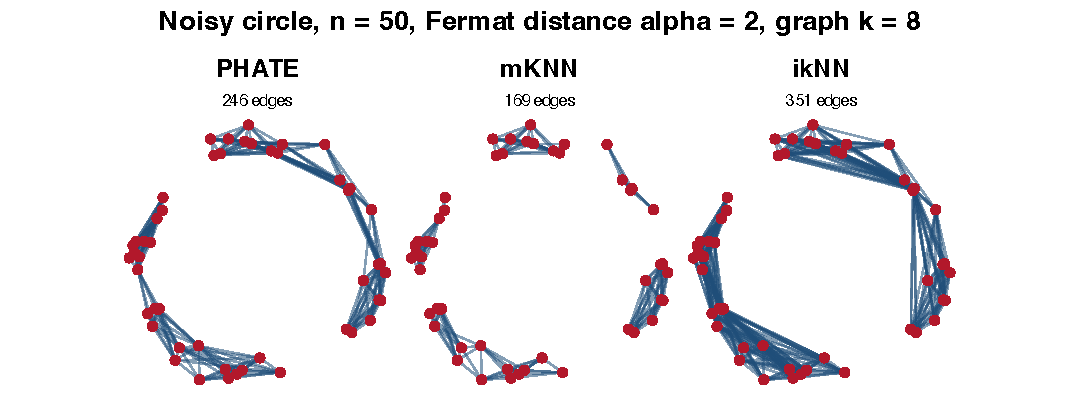
\includegraphics[width=\linewidth]{figures/noisy_circle_fermat_n50_k8.pdf}
  \caption{Noisy circle, \(n=50\), graph \(k=8\), sample Fermat distance with \(\alpha=2\).}
\end{figure}

\begin{figure}[htbp]
  \centering
  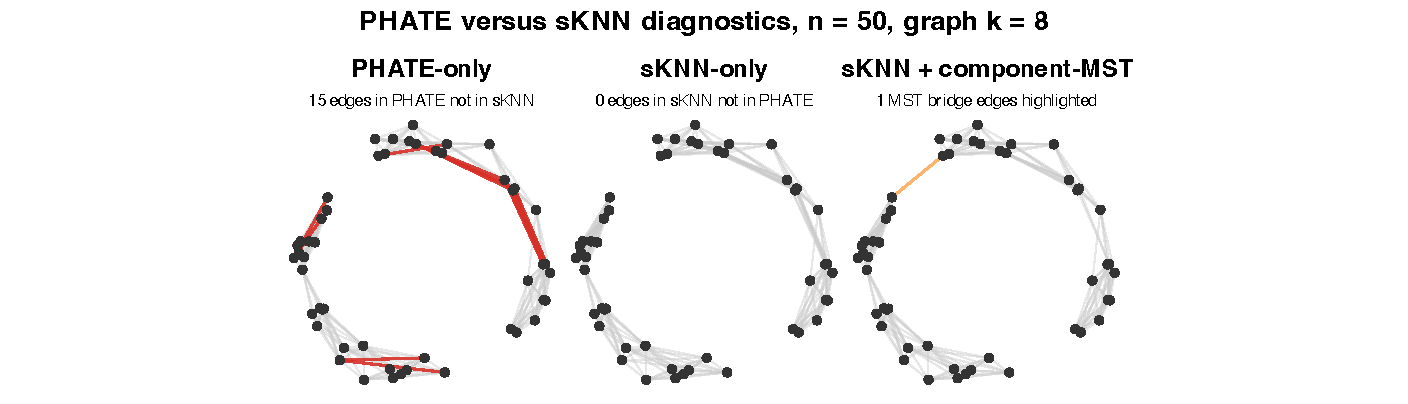
\includegraphics[width=\linewidth]{figures/noisy_circle_fermat_n50_k8_diagnostics.pdf}
  \caption{Noisy circle, \(n=50\), PHATE-versus-sKNN diagnostics.}
\end{figure}

\begin{figure}[htbp]
  \centering
  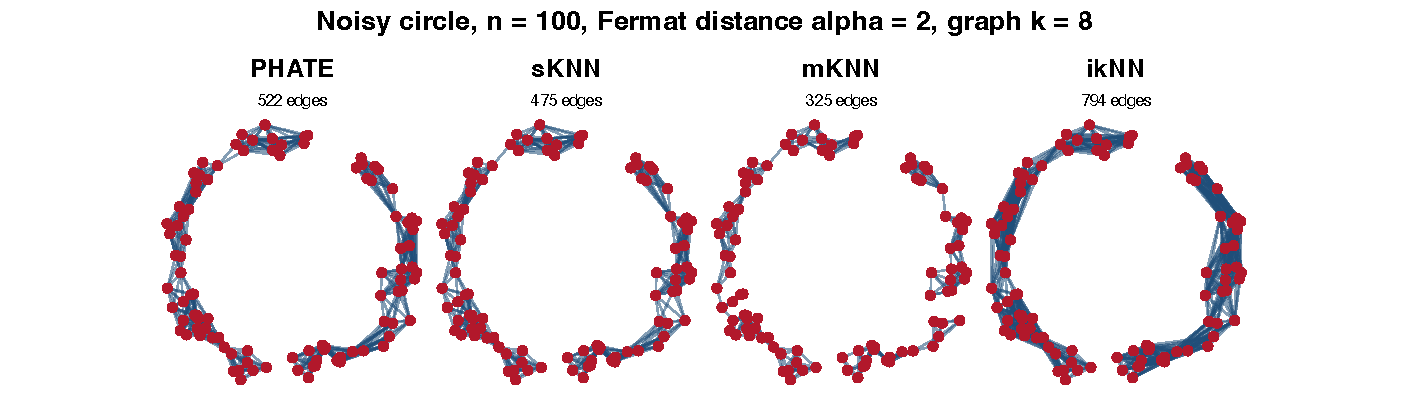
\includegraphics[width=\linewidth]{figures/noisy_circle_fermat_n100_k8.pdf}
  \caption{Noisy circle, \(n=100\), graph \(k=8\), sample Fermat distance with \(\alpha=2\).}
\end{figure}

\begin{figure}[htbp]
  \centering
  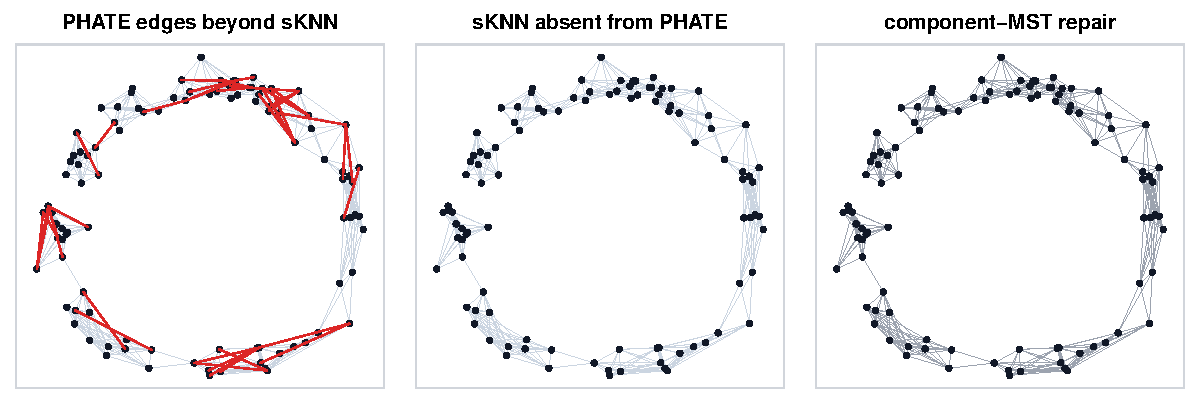
\includegraphics[width=\linewidth]{figures/noisy_circle_fermat_n100_k8_diagnostics.pdf}
  \caption{Noisy circle, \(n=100\), PHATE-versus-sKNN diagnostics.}
\end{figure}

\begin{figure}[htbp]
  \centering
  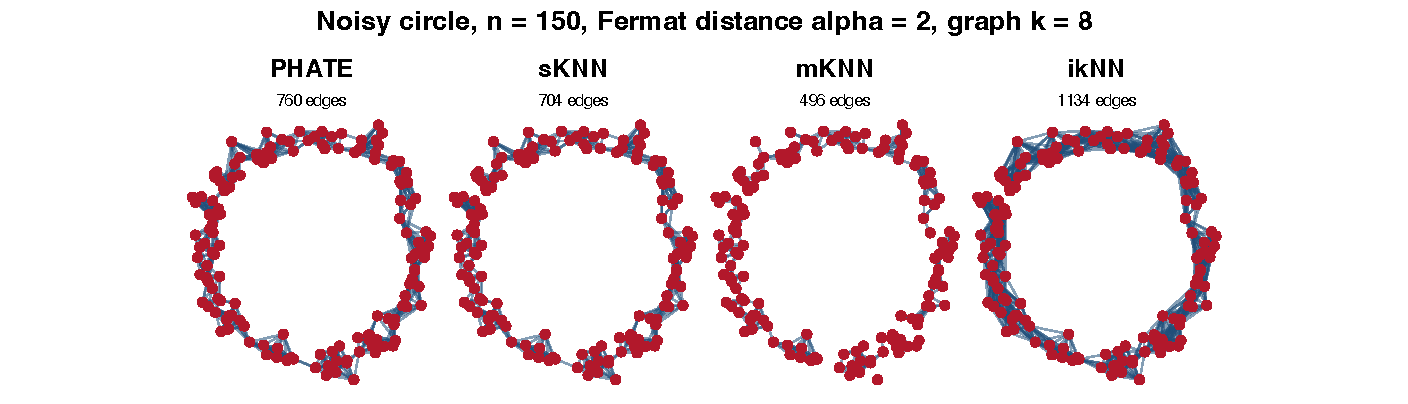
\includegraphics[width=\linewidth]{figures/noisy_circle_fermat_n150_k8.pdf}
  \caption{Noisy circle, \(n=150\), graph \(k=8\), sample Fermat distance with \(\alpha=2\).}
\end{figure}

\begin{figure}[htbp]
  \centering
  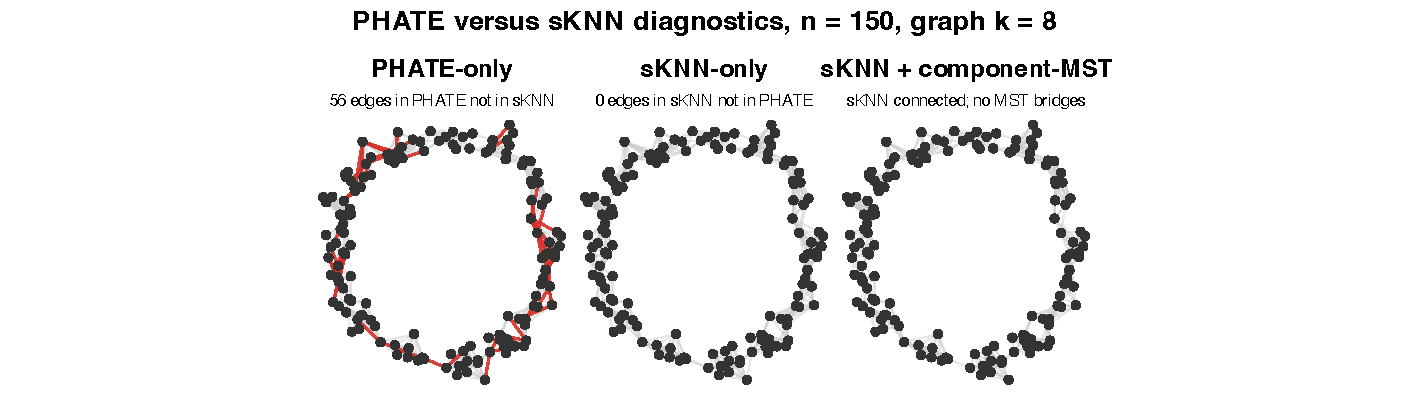
\includegraphics[width=\linewidth]{figures/noisy_circle_fermat_n150_k8_diagnostics.pdf}
  \caption{Noisy circle, \(n=150\), PHATE-versus-sKNN diagnostics.}
\end{figure}

\section{Summary}

The graph constructions answer different local questions:
\begin{itemize}[leftmargin=2em]
  \item mKNN asks whether two points are reciprocal nearest neighbors:
  \[
    d_{ij}\le\min(\sigma_i,\sigma_j).
  \]
  \item sKNN/uKNN asks whether at least one endpoint has the other as a k-nearest neighbor:
  \[
    d_{ij}\le\max(\sigma_i,\sigma_j).
  \]
  \item PHATE asks whether at least one endpoint sees the other within its adaptive
  threshold radius:
  \[
    d_{ij}\le r_\tau\max(\sigma_i,\sigma_j).
  \]
  \item ikNN asks whether two points share at least one point in their closed neighborhoods:
  \[
    \widehat{N}_k(i)\cap \widehat{N}_k(j)\ne\varnothing.
  \]
\end{itemize}
Thus mKNN is contained in sKNN, sKNN is contained in PHATE when \(r_\tau\ge 1\), and mKNN is
also contained in closed-neighborhood ikNN.  PHATE and ikNN are not generally nested.  In
many data examples ikNN is denser, but the relationship is not merely an edge-count
hierarchy.  This distinction matters when the goal is geodesic reconstruction: PHATE support
may improve local geometric connectivity even when its support is sparser than ikNN, while
ikNN may introduce shared-neighborhood edges that are not direct adaptive-radius edges.

\section*{References}

\begin{enumerate}[leftmargin=2em]
  \item K. R. Moon, D. van Dijk, Z. Wang, S. Gigante, D. B. Burkhardt, W. S. Chen,
  K. Yim, A. van den Elzen, M. J. Hirn, R. R. Coifman, N. B. Ivanova, G. Wolf,
  and S. Krishnaswamy. ``Visualizing structure and transitions in high-dimensional
  biological data.'' \emph{Nature Biotechnology}, 2019.  PHATE introduced the
  adaptive affinity and diffusion-potential embedding pipeline.
  \item D. Groisman, M. Jonckheere, and F. Sapienza. ``Nonhomogeneous Euclidean
  first-passage percolation and distance learning.'' arXiv:1810.09398.  This work
  uses the name Fermat distance for the continuum limit of sample shortest-path
  distances with powered edge costs.
  \item N. García Trillos, M. Gerlach, M. Hein, and D. Slepčev. ``Fermat Distances:
  Metric Approximation, Spectral Convergence, and Clustering Algorithms.''
  \emph{Journal of Machine Learning Research}, 2024.  This paper studies discrete
  sample Fermat distances and related graph Laplacians.
  \item M. Maier, U. von Luxburg, and M. Hein. ``Influence of graph construction on
  graph-based clustering measures.'' \emph{Advances in Neural Information Processing
  Systems}, 2009.  This work discusses symmetric and mutual kNN graph constructions
  in graph-based clustering.
  \item L. McInnes, J. Healy, and J. Melville. ``UMAP: Uniform Manifold Approximation
  and Projection for Dimension Reduction.'' arXiv:1802.03426.  UMAP combines directed
  local neighbor memberships through a fuzzy union.
  \item T. Stuart, A. Butler, P. Hoffman, C. Hafemeister, E. Papalexi, W. M. Mauck III,
  Y. Hao, M. Stoeckius, P. Smibert, and R. Satija. ``Comprehensive Integration of
  Single-Cell Data.'' \emph{Cell}, 2019.  The Seurat workflow uses kNN and SNN graph
  constructions for single-cell analysis.
  \item P. Veenstra, C. Cooper, and S. Phelps. ``Spectral clustering using the
  kNN-MST similarity graph.'' \emph{CEEC}, 2016.  This paper uses the union of a
  kNN graph and a minimum spanning tree as a connected similarity graph for spectral
  clustering.
\end{enumerate}

\end{document}
